
\chapter{State of the art and Problem definition}
\label{cha:state_of_the_art_and_problem_definition}

\graphicspath{{Chapter1-State-of-the-art/Figs/}}

\section{State of the art}
\label{sec:state_of_the_art}

\subsection{Inverse Kinematics}
\label{sub:inverse_kinematics}

Posture generation can be viewed as, and is sometimes called, Generalized Inverse Kinematics.
The Inverse Kinematics~(IK) problem consists of finding the joint configuration for an articulated multibody system in order to complete a given set of tasks that are defined in the operational space.
For example, by solving repeatedly the IK for a desired motion given in the Cartesian space, we can generate motions in the joint space.
By definition, such a process is purely kinematics. But other constraints need dynamic or other physics-related knowledge such as the inertia or contact friction parameters.
The IK problem has been widely studied and used in the fields of robotics, computer graphics and games, and animation.
In few particular cases, for example with robotic arms that have less than 7 degrees of freedom, a closed-form solution can be found.
For example, in~\cite{asfour2003human} the redundancy in a robot arm is exploited to derive a closed-form formula for its IK.
However, for most complex cases, iterative methods are required.

%Generating desired initial, intermediary or finale posture configurations requires defining static task goals (e.g.\ reach a target point in 6D) to be done under intrinsic constraints such as joint limits, torque limits, avoiding non-desired self-collisions\ldots and perceptual or extrinsic ones such as keeping an object in the embedded camera field-of-view, avoiding non-desired collisions with surrounding objects, etc.

Many approaches to solve IK problems use pseudo-inverse or Gauss-Newton method with the Jacobian, Jacobian transpose, damped least squares with or without singular values decomposition or selectively damped least squares~\cite{balestrino1984robust, tolani2000real, baillieul1985kinematic, wampler1986manipulator, nakamura1986inverse, buss2005selectively}.
These approaches are all computationally costly and suffer from joint-space and workspace singularities~\cite{aristidou2009inverse}.

In~\cite{pechev2008inverse} an alternative method based on a control approach is proposed, where no matrix manipulation is required, this approach is as fast as the damped least squares, but outperforms them in terms of handling singularities.
The closed-loop inverse kinematics scheme presented in~\cite{siciliano1990closed} is a well-known approach to solve IK problems in a control context, and uses a second order tracking scheme to guarantee satisfactory tracking performance.

Handling conflicting constraints in IK is a challenging problem to which \cite{baerlocher2004inverse} and \cite{sentis2005synthesis} propose solutions by enforcing a number of priority levels among constraints in their resolution schemes to generate whole-body control of complex articulated figures.

Other stochastic approaches such as sequential Monte Carlo \cite{courty2008inverse} and a particle filtering \cite{hecker2008real} have the advantage that they only use direct calculations and never require matrix inversions.
They perform particularly well compared to other methods when solving problems with high numbers of degrees of freedom.

In~\cite{AristidouFABRIK, Aristidou:2016_ExtFABRIK} the forward and backward reaching inverse kinematics (FABRIK) resolution method is introduced.
This method is based on a geometric iterative heuristic approach, where the bodies of a robot are moved iteratively and separately to reach a target with the end effector while maintaining the integrity of the robot's structure.
This approach is simple to implement, does not suffer from singularities and requires fewer iterations than most other IK methods.
But it cannot easily be extended to take non-geometric constraints into account.

Finding an acceptable approximate (or a probabilistic) solution to an IK problem without any regard for its stability is a common approach in the field of randomized path planning.
\cite{cortes2002random} proposes a method to generate many random configurations for closed loop systems with an increased probability that they are kinematically valid in terms of closure constraints.
These configurations are then used in the construction of a Probabilistic RoadMap.
In~\cite{lavalle1999probabilistic}, a similar approach is presented, where the closure constraint is enforced for each configuration by additional treatment.

\subsection{Generalized Inverse Kinematics}
\label{sub:generalized_inverse_kinematics}

The term Generalized Inverse Kinematics refers to a problem similar to the Inverse Kinematics in the sense that it searches for a joint configuration for an articulated figure to achieve goal tasks, but needs to do so under various constraints, like ensuring the equilibrium stability of the structure, respecting its torque limits, avoiding collisions with the environment or with itself, etc.

All the previously mentioned approaches are used to find a robot configuration solution to the geometric IK problem.
To solve a Generalized Inverse Kinematics problem with stability constraints, one can first solve the associated IK with one of the methods presented above, and then test the stability of the IK solution, using methods such as the ones presented in~\cite{bretl:itro:2008} or~\cite{rimon2008general} that determine if the configuration can be statically stable.
This gives a rejection criterion for a proposed solution.
If the solution can be stable, the optimal contact forces can be computed using the method proposed in~\cite{boyd2007fast} (which in turn allows computing the joint torques).
Otherwise, another IK solution is generated and tested.
And the process is repeated until a satisfactory solution is found.
This type of sequential approach for the resolution of a posture generation problem features a rejection criterion that can, in some cases, be difficult to overcome, making this approach costly, for example, if there is a small number of contacts and very few configurations are stable.

%Those approach lead to a sequential resolution of the posture generation problem where a solution to the IK problem is searched, then tested for stability, if it is stable, the optimal forces are computed, otherwise, another solution is searched for.

Another way to solve the posture generation problem is to consider the complete problem at once, with the IK targets and all the other constraints (stability, collisions, torque limits, etc.) in a single nonlinear constrained optimization problem.
This approach is used in~\cite{Zhao1994} to solve the IK problem.
That is the approach that we and many others use to solve Generalized Inverse Kinematics problems.
In~\cite{escande:iros:2006}, such an approach is employed to generate postures that are used to grow a tree of usable postures in a multi-contact planning algorithm.
\cite{escande:iros:2006} applied the approach to automatically generate a sequence of contact sets and postures where the HRP-2 robot uses its hand to lean on a table in order to grasp an object otherwise out of reach.
Interestingly, in this study, the C-code that computes the robot's kinematics is generated once and for all for each robot, using Maple and the HuMAnS toolbox~\cite{wieber2006humans} provided by INRIA.
The constraints of contact, stability and collision are then computed based on the outputs of the generated code.
And the problem is solved by the CFSQP solver~\cite{cfsqp:manual}.
In~\cite{hauser:ijrr:2008}, a similar posture generation approach is used to find viable postures for different legged robots on varied terrains in the context of Probabilistic RoadMap planning, which is a planning approach based on random sampling of the configuration space.
%\cite{hauser:issr:2007} presents a different approach to multi-contact planning based on probabilistic roadmap and random sampling of the configuration space.
In~\cite{bouyarmane2010static}, a generalization of the formulation of posture generation problems for systems of multiple robots and manipulated objects is proposed.
%In this formulation, the notion of contacts is generalized to bear forces or not and to have any orientation.
With this formulation, the notion of contacts is generalized such that they are not necessarily coplanar, nor necessarily horizontal, frictional, can bear forces or not, and may be unilateral or bilateral.
This generic formulation enables the generation of postures with inter-robot contacts.
The complete posture generation problem is then solved within a single nonlinear constrained optimization query, computing the contact forces and joint configuration at the same time, while ensuring the stability of all the `robotic agents', avoiding collision and respecting the robot's joint and torque limits.

In the past few years, our team has dedicated considerable efforts in proposing a general multi-contact motion planner to solve cases of non-gaited acyclic planning, using a posture generator as a backbone to select valid configurations.
Given a humanoid robot, an environment, a start and a final desired postures, the planner generates a sequence of contact stances allowing any part of the humanoid to make contact with any part of the environment to achieve motion towards the goal.
The planner's role is to grow a tree of contact stances iteratively; from a given posture, it tries to add or remove contacts one by one.
The tree grows following some heuristics until the solution is reached.
For each set of contacts to add to the tree, a posture generation problem is solved in order to validate the feasibility of the set. If it is not feasible, the set is rejected.
A typical experiment with an HRP-2 robot achieving such an acyclic motion is presented in~\cite{escande:iser:2008}, and the planner is thoroughly described in~\cite{escande:ras:2013}.
Extensions of this multi-contact planner to multi-agent robots and objects gathering locomotion and manipulation are presented in~\cite{bouyarmane:ar:2012}, and preliminary validations with some DARPA challenge scenarios, such as climbing a ladder, ingress/egress a utility car, or crossing through a relatively constrained pathway are presented in~\cite{bouyarmane:humanoids:2012}.
Another way of planning a multi-contact scenario, which is actually often used when planners fail to find satisfactory solutions, is manual, choosing iteratively which contacts to add and remove until the goal is reached.
This type of approach is used when the plan to execute is complex and when a lot of fine tuning of the postures is required, as in~\cite{vaillant:autonomousrobots:2016}, where a sequence of postures allowing the HRP-2 robot to climb a vertical ladder is generated and tuned manually.
Those postures are provided as input to a finite state machine that builds additional intermediary tasks and specific grasps procedures to be realized on the real robot by a multi-objective model-based QP controller.

Instead of feeding the key postures directly to the controller and trusting that it will find a path to connect them, one can take an additional step and compute a dynamically viable trajectory between successive steps that the controller will then have to follow.
Classical methods generate satisfactory configurations on a discretized time-grid and then extrapolate the motion between configurations at successive time-grid points.
This approach does not guarantee that the constraints are satisfied at every point of a continuous time interval, which is dangerous for the robot.
Interval analysis methods can be leveraged to compute safe motions over continuous time intervals, as proposed in~\cite{lengagne2011planning}.
This work was extended in~\cite{lengagne2013generation} to generate whole-body multi-contact dynamic motions.
The constraints are transformed into a computation of extrema of time polynomials, whose coefficients are a function of the optimization variables, over each time interval.
Generating full body dynamic motions allows one to take advantage of the dynamic effects and to produce motions with better performances in terms of completion time, energy consumption, or other criterions.

In many planning approaches~\cite{kuffner2005motion, chestnutt2007navigation, hauser:ijrr:2008, kolter2008control, bouyarmane:icra:2011} the planning problem is decomposed into two stages, first the sets of contacts and associated postures are planned and then the motions to go from one set to another are computed.
These two stages are loosely coupled, which can result in suboptimal use of the contacts available.
\cite{mordatch:acm:2012} presents a different approach to contact planning where some additional terms and variables are added to the optimization problem to decide whether a contact pair should be active (and bear forces) at any given time during the motion, or not.
The contact sets, as well as the postures associated, are discovered along with the entire movement's trajectories by using contact invariant optimization.
This allows for the exploitation of any synergies that might exist between the contact events and the motion trajectory.

In~\cite{tonneauijrr16}, a multi-contact planning framework is presented that allows the computation of complex multi-contact motions in very short times.
It is based on several heuristics that allow fast computations of the motions.
Starting by generating a guide path that satisfies the reachability condition, which means that the root body is close to obstacles to allow making contacts with them but not too close to avoid collisions.
A discrete sequence of statically stable whole-body configurations along this path is then generated efficiently by taking advantage of several approximations and heuristics.
This approach allows generating complex contact plans in a few seconds, whereas other approaches usually take several minutes.

In~\cite{liu:acm:2012}, posture generation is used to find the optimal posture and position of contacts to optimally realize a manipulation task along a path while satisfying geometric, kinematic, as well as force and torque constraints.
The task is defined as a path and forces to follow with an end effector.
Instead of finding a sequence of unrelated postures along the path, all the postures are found by solving a single optimization problem in which successive postures are coupled by constraints to ensure that the foot positions remain constant during the task, even though the rest of the body can move.
This approach allows the robot or virtual character to apply manipulation forces as strongly as possible while avoiding foot slippage.
It also allows taking external perturbations into account to generate more robust postures.

A different utilization of the posture generation was presented in~\cite{stasse:humanoids:2007}, that deals with the problem of object reconstruction.
An object is presented to the robot in order to generate automatically its 3D model.
To do so, the object is observed from several different angles with the camera that is mounted in the robot's head.
The satisfactory postures of the robot to complete this task are obtained by solving a posture generation problem to which a set of constraints defining the direction in which the robot should look and a minimum distance from the object are added.
While in this work the observation directions are predefined,~\cite{foissotte:humanoids:2008} presents an approach where the choice of the best observation direction is left to the posture generator.
The representation of the object is iteratively carved into a block of 3D voxels, each new point-of-view chosen to allow to carve it a little more precisely.
It uses a modified cost function to evaluate the amount of information on the object that a given point of view can provide.
The posture of the robot that optimizes that cost function is then found by the posture generator under the classical constraints of stability, collision avoidance, and other robot's limitations.


\subsection{Optimization}
\label{sub:optimization}

The resolution of a posture generation problem is often done by solving a nonlinear optimization problem which consists of finding the optimal point that minimizes a cost function and maybe constraints, the cost and constraints functions being possibly nonlinear.

Optimization algorithms can be derivative-free or not.
The computation of the derivatives of the functions involved in the problem is a common source of error.
The strength of the derivative-free approaches is that the user does not need to implement the derivatives.
But derivative-free approaches are much slower than their counterparts using derivatives.
One way to avoid implementation errors in the derivatives computation is to use finite differences to compute them.
This method is very slow, especially when the dimension of the problem is large.
In order to design an efficient optimization algorithm, we will focus on methods using derivative information and will implement those derivatives' computations.
The finite difference approach can be used to verify the correctness of the computed derivative.

Nonlinear optimization is a well-established research field by its own and has been extensively studied in the past and nowadays.
One can find some excellent reference books about optimization, such as~\cite{nocedal:book:2006, bonnans:book:2003, boyd2004convex}.

Furthermore, several off-the-shelf solvers are available and have been widely used to solve robotics problems.
The CFSQP solver~\cite{cfsqp:manual} was used in~\cite{escande:iros:2009} and~\cite{escande:ras:2013} where thousands of HRP-2 posture generation queries were made to explore the feasible space.
The IPOPT solver~\cite{wachter:mathprog:2006} has been used in~\cite{vaillant:humanoids:2014},~\cite{vaillant:autonomousrobots:2016},~\cite{bouyarmane:ar:2012} where the posture generator has been extended to handle multi-robot problems with more complex and various contact constraints.
The SNOPT solver~\cite{gill2005snopt} was used in~\cite{dai2014whole} to plan dynamic whole-body trajectories.
Several nonlinear optimization solvers are available and have been packaged for use in robotics problems in the Roboptim Framework~\cite{moulard:jsme:2013}, such as IPOPT, CFSQP, CMinPack~\cite{cminpack}, NAG~\cite{nag}, KNITRO~\cite{knitro} and PGSolver (the solver that we develop in this thesis).

Traditionally, optimization problems are solved over Euclidean spaces.
When the need comes to find a solution to an optimization problem in a non-Euclidean space $\mathcal{M}$, the commonly used method is to represent the elements of $\mathcal{M}$ in a Euclidean manifold of higher dimension, and enforcing that solution of the optimization problem should lie on $\mathcal{M}$ by adding the necessary constraints to the problem.
We will detail the drawbacks of such approaches in Chapter~\ref{chapter:optimization_on_noneuclidean_manifolds}.
Alternatively, there exists a method to run an optimization algorithm directly on a non-Euclidean manifold, as it is presented in great detail in the book~\cite{absil:book:2008}.
A non-Euclidean manifold can be thought of as a space that is locally Euclidean, but is not so globally.
For example, a sphere looks Euclidean if one examines a small-enough neighborhood, similar to the surface of a giant sphere like the earth that looks flat for a human being standing on it.
Based on the fact that manifolds are locally Euclidean, the classic properties of distance, derivatives, and in general all the Euclidean geometry can be used locally.
Based on that property, several optimization methods traditionally used on Euclidean manifolds have been extended to non-Euclidean manifolds.
The gradient methods have been extended to manifolds in~\cite{luenberger1972gradient, gabay1982minimizing}.
The Newton methods on manifolds which have better convergence rates were extended to manifolds in~\cite{gabay1982minimizing, stuart1998dynamical, smith2013geometric}.
And Quasi-Newton methods in~\cite{gabay1982minimizing}.
Those approaches are only meant to solve unconstrained optimization problems, which is not enough to solve posture generation problems, where the presence of constraints is unavoidable.

The main idea to optimize on manifolds is that we use a local map between the neighborhood of the current iterate and its Euclidean tangent space in order to run an optimization step and choose an increment in the tangent space that is mapped back to the manifold.
Once the iterate has been incremented, the process is repeated with the map and tangent space associated with the new iterate.
This comes down to re-parameterizing the problem around the current iterate at each iteration.

In the field of robotics, we are only aware of the work of Schulman~\emph{et al.}~\cite{Schulman2014}, where the authors explain the adaptation of their solver to work on $SE(3)$.
In the field of computer vision, and especially for solving pose estimation problems, optimization on manifolds is used often, e.g.~\cite{hertzberg2011, lu2000fast}.

In this thesis, we develop a nonlinear solver on manifolds that can handle constraints.
We were largely inspired by the work of Fletcher concerning the notions of `Sequential Quadratic Programming without a penalty function' ~\cite{Fletcher:ifip:2006, fletcher2010sequential, fletcher:mathprog:2000}, along with other optimization approaches that we adapted to work with manifolds.

\section{Problem Definition}
\label{sec:problem_definition}

%%%%%%%%%%%%%%%%%%%%%%%%%%%%%%%%%%%%%%%%%%%%%%%%%%%%%%%%%%%%%%%%%%%%%%%
%                     SECTION PROBLEM DEFINITION                      %
%%%%%%%%%%%%%%%%%%%%%%%%%%%%%%%%%%%%%%%%%%%%%%%%%%%%%%%%%%%%%%%%%%%%%%%

We consider the problem where we have a robotic system and we want it to realize a set of tasks $T_i$.
We denote $\bf q$ as the joint configuration ($n$ joints + base) of the robot and $\mathbf{f} =\{\mathbf{f}_i\,, i\in[1,m]\}$ represents the $m$ contact forces applied on the robot.
Each task $T_i$ can be represented by a set of equality and inequality equations:
\begin{equation}
  \left\{
    \begin{aligned}
    g_i(\mathbf{q},\mathbf{f}) = 0\\
    h_i(\mathbf{q},\mathbf{f}) \geq 0
    \end{aligned}
  \right.
\end{equation}
For example, the task of making contact between a body (link) of the robot and a part of the environment can be represented in such a way.

In addition to satisfying the tasks $T_i$, the solution configuration to our problem must describe a viable posture of the robotic system, in the sense that it ensures its integrity.
Which translates into the following list of constraints.
It must respect the joint limits of the robot~\eqref{subeq:bounds}, as well as its torque limits~\eqref{subeq:tau}.
Equation~\eqref{subeq:autocoll} translates the auto-collision avoidance constraint between a pair of bodies $\{r_i, r_j\}$ given by a set $\mathcal{I}_\text{auto}$ where $d$ is the minimal distance between two bodies.
Equation~\eqref{subeq:coll} denotes the collision avoidance constraint between a robot body $r_i$ and an object of the environment $O_k$ defined in a set $\mathcal{I}_\text{coll}$.
$\epsilon_{ij}$ and $\epsilon_{ik}$ denote the smallest acceptable distance for their respective constraints.
The stability of the robot is ensured by the respect of equation~\eqref{subeq:stab}, which is the Euler-Newton equation(or a simplification of it).
To avoid slippage of the contacts, the contact forces must remain in the Coulomb friction cones, which is enforced by equation~\eqref{subeq:friction}.
Equations~\eqref{subeq:gi} and~\eqref{subeq:hi} translate the constraints to satisfy task $T_i$.

The set of satisfying configurations can be defined by $\mathcal{Q}$:

\begin{empheq}[left={\mathcal{Q}=\{\mathbf{q}, \mathbf{f}\}:\empheqlbrace}]{align}
      & q_i^- \leq q_i \leq q_i^+ \quad \forall i\in[1,n] & \text{joint limits} \label{subeq:bounds}\\
      & \tau_i^- \leq \tau_i(\mathbf{q}, \mathbf{f}) \leq \tau_i^+ \quad \forall i\in[1,n] & \text{torque limits}\label{subeq:tau}\\
      & \epsilon_{ij} \leq d(r_i(\mathbf{q}), r_j(\mathbf{q})),\quad \forall (i,j)\in\mathcal{I}_\text{auto} & \text{auto-collision}\label{subeq:autocoll}\\
      & \epsilon_{ik} \leq d(r_i(\mathbf{q}), O_k),\quad \forall (i,k)\in\mathcal{I}_\text{coll} & \text{collision}\label{subeq:coll}\\
      & s(\mathbf{q}, \mathbf{f}) = 0 & \text{stability} \label{subeq:stab}\\
      & c(\mathbf{f}_i) \geq 0 \quad i\in[1,m] & \text{slippage avoidance} \label{subeq:friction}\\
      & g_i(\mathbf{q}, \mathbf{f}) = 0 & \text{task i's equalities}\label{subeq:gi}\\
      & h_i(\mathbf{q}, \mathbf{f}) \geq 0 & \text{task i's inequalities} \label{subeq:hi}
\end{empheq}

We illustrate these constraints in~\Figref{fig:PG} and will explain them in more details in Chapter~\ref{cha:posture_generation_problem_formulation}.

%Where inequalities~\eqref{subeq:bounds} represent the joint limits, and~\eqref{subeq:tau} the torque limits.

\begin{figure}[ht]
  \centering
  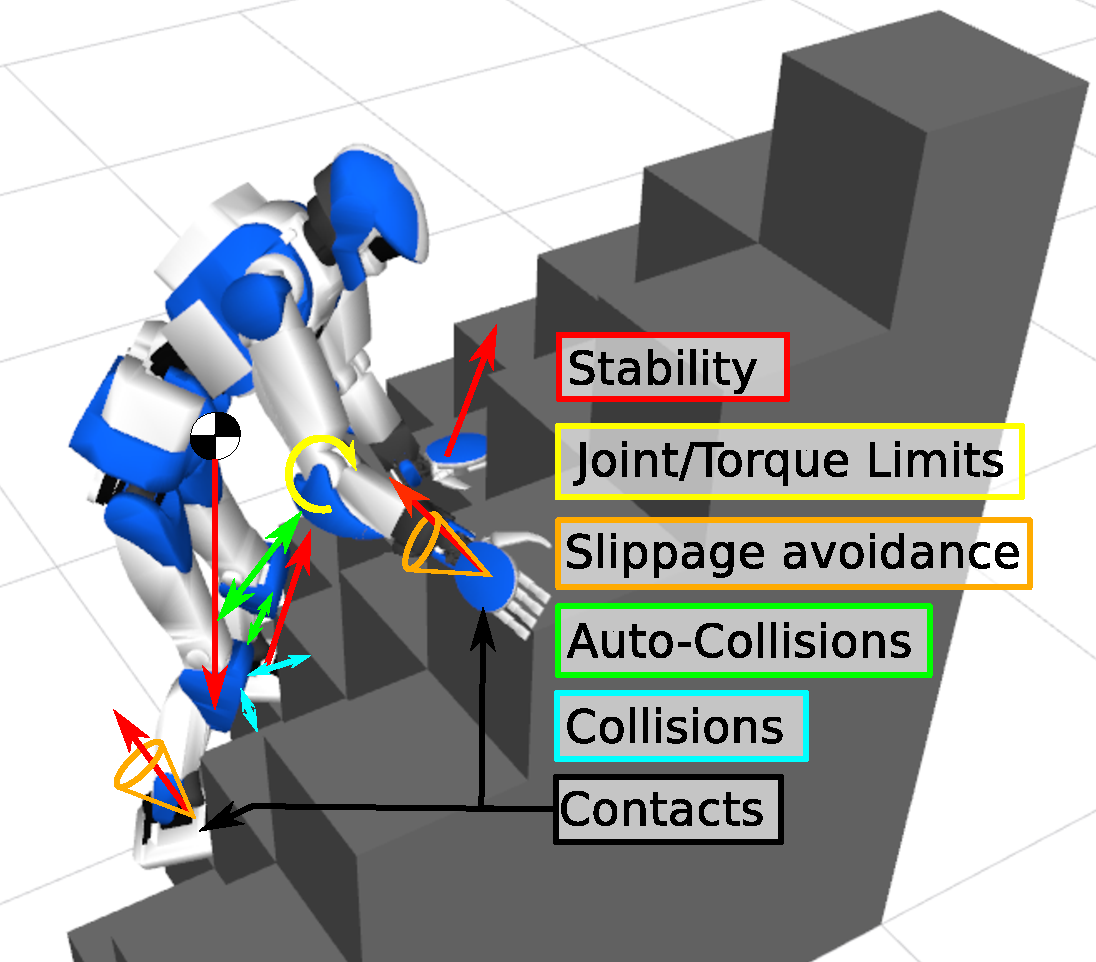
\includegraphics[width=0.7\textwidth]{PG.pdf}
  \caption{The HRP-4 on a stack of cubes. The color of each box corresponds to the color of the constraint it depicts.}
\label{fig:PG}
\end{figure}

In addition to satisfying the set of constraints $T_i$, one can require the searched posture to be optimal in the sense of some cost function $f$.
Defining a cost function can help the user control the result of the problem; for example, by minimizing the distance to a reference posture or maximizing the contact force applied by one end-effector.
In~\cite{escande2009} the cost function was used to guide the posture toward the end of a planning problem.
A sum of different criterions can be used as cost function.
The optimization problem that describes the posture generation problem becomes:


%We consider the problem where we have a robotic system and we want it to do some tasks, like for example to make a contact between a point on a body of the robot and a point of the environment.
%This contact task can be modelized as a simple equality.
%We denote $q$ the joint configuration (joint + base) of the robot, $g(q)$ is the 3D position of the point of interest on the robot and $P$ is the point of the environment.
%Then our problem comes down to finding a configuration $q^*$ such that $g(q^*) = P$.
%For robots like humanoids, the equations describing their kinematics are quite complicated, and, in the presence of angular joints, they are nonlinear.
%In the general case, even for simple tasks, a closed form solution of the problem does not exist.

%We denote $\mathcal{C}$ the configuration space of our robotic system.
%It is the manifold in which $q$ lives. The dimension of $\mathcal{C}$ is equal to the number of degrees of freedom of the robot.
%Note that if all the joints of the robot are actuated, this is the number of motors of the robot.
%And if the robot has a free-floating basis (is not fixed) then the position in $\mathbb{R}^3$ and rotation in $SO(3)$ of its basis are part of $q$.

%We can formulate that problem as follows:

%\begin{equation}
  %\text{find}\ q\in\mathcal{C}\ \text{such that}\ g(q)=P
%\end{equation}

%The space of solution of this problem is a submanifold of $\mathcal{C}$ that we call ${\mathcal{C}}_F$ the feasible configuration space (which can be empty).

%In addition to the equality constraint abovementioned, the problem can feature some inequality constraints.
%For example, each joint variable can be limited to a certain range of value: $\forall i,\ q_i\in [q_i^-,\ q_i^+]$.
%Then the problem becomes a combination of equality and inequality constraints.%, and can be written as:
%%\begin{equation}
  %%\text{find}\ q\in\mathcal{C}\ \text{such that}\left\{
  %%\begin{array}{l}
    %%g(q)=P \\
    %%\forall i,\ q_i^- \leq q_i \leq q_i^+
  %%\end{array}
  %%\right.
%%\end{equation}
%Finally, we can also require finding the point of $\mathcal{C}_F$ that minimizes a criterion, such as the distance to a goal posture $q_0$.
%Our problem becomes:

%\begin{equation}
  %\left\{
  %\begin{array}{l}
    %\minimize\limits_{q\in\mathcal{C}}{\|q-q_0\|_2}\\
    %\text{ s.t. }
    %\left\{
    %\begin{array}{l}
      %g(q)=P\\
      %\forall i,\ q_i^- \leq q_i \leq q_i^+
    %\end{array}
    %\right.
  %\end{array}
  %\right.
%\end{equation}

\begin{equation}
  \begin{array}{l}
    \minimize\limits_{\mathbf{q}, \mathbf{f}}{f(\mathbf{q}, \mathbf{f})}\\
    \text{ s.t. }\{\mathbf{q}, \mathbf{f}\}\in\mathcal{Q}
  \end{array}
\end{equation}

This type of problem is called a nonlinear constrained optimization problem and can be formulated in a more generic fashion as:

\begin{equation}
\label{eq:optim_form_PG}
  \begin{array}{l}
    \minimize\limits_{x}{f(x)}\\
    \text{ s.t. }
    \left\{
    \begin{array}{l}
      c_i(x) = 0,\ \forall i\in{E}\\
      c_i(x) \geq 0,\ \forall i\in{I}\\
    \end{array}
    \right.
  \end{array}
\end{equation}
where $x$ is the optimization variable, that we want to find, and which minimizes the cost function $f(x)$ while satisfying the equality constraints $c_i(x) = 0,\ \forall i\in{E}$ and inequality constraints $c_i(x) \geq 0,\ \forall i\in{I}$.
Such problems can be solved by a nonlinear optimization solver.
In Appendix~\ref{chapter:optimization}, we present some classical concepts of nonlinear optimization.
%Several off-the-shelf solvers are available and have been widely used in for solving robotics problems.
%The CFSQP solver~\cite{cfsqp:manual} was used in~\cite{escande:iros:2009} and~\cite{escande:ras:2013} where thousands of HRP-2 posture generation queries were made to explore the feasible space.
%The IPOPT solver~\cite{wachter:mathprog:2006} has been used in~\cite{vaillant:humanoids:2014},~\cite{vaillant:autonomousrobots:2016},~\cite{bouyarmane:ar:2012} where the posture generator had been extended to handle multi-robot problems and more complex and various contact models.
%The SNOPT solver~\cite{gill2005snopt} was used in~\cite{dai2014whole} to plan dynamic whole-body trajectories.
%Several nonlinear optimization solvers are available and have been packaged for use in robotics problems in the Roboptim Framework~\cite{moulard:jsme:2013}, such as IPOPT, CFSQP, CMinPack~\cite{cminpack}, NAG~\cite{nag}, KNITRO~\cite{knitro} and PGSolver, the solver that we develop in this thesis.

In this thesis, we used the off-the-shelf solver IPOPT~\cite{wachter:mathprog:2006} in the beginning.
At a later stage, we developed and use our own nonlinear solver called {\tt PGSolver}.
From here on, we will formulate and solve posture generation problems as nonlinear constrained optimization problems.
In the next chapter, we focus on formulating all the basic functions and algorithms used to describe the robotic constraints and cost function in the formalism of nonlinear optimization.
